\documentclass[11pt]{article}

\usepackage[a4paper,margin=1in]{geometry}
\usepackage{amsmath,amssymb,mathtools}
\usepackage{array}
\usepackage{booktabs}
\usepackage{enumitem}
\usepackage[hidelinks]{hyperref}
\usepackage{xcolor}
\usepackage{tikz}
\usepackage{listings}

\setlength{\emergencystretch}{3em}

\newcommand{\code}[1]{\texttt{\detokenize{#1}}}
\newcommand{\Phat}{\mathbb P}
\newcommand{\Khat}{\widehat K}
\newcommand{\dd}{\,\mathrm d}
\newcommand{\grad}{\nabla}
\newcommand{\lam}{\lambda}

\lstset{
  basicstyle=\ttfamily\small,
  columns=fullflexible,
  keepspaces=true,
  frame=single,
  breaklines=true,
  backgroundcolor=\color{black!3}
}

\title{Symmetric Triangle Quadrature in HYBRIDGE}
\author{}
\date{}

\begin{document}
\maketitle

\begin{abstract}
This note derives the symmetric triangle quadrature policy and its validation
requirements. It explains why degree \(2p\) appears in diffusion assembly and
why collapsed-coordinate implementation formulas still represent polynomial
bases despite removable singularities.
\end{abstract}

\tableofcontents

\section{Reference triangle}

HYBRIDGE uses the reference triangle
\[
  \Khat = \operatorname{conv}\{(-1,-1), (1,-1), (-1,1)\}.
\]
For a point \((\xi,\eta)\in\Khat\), the barycentric coordinates are
\[
  \lam_1 = \frac{\xi+1}{2},\qquad
  \lam_2 = \frac{\eta+1}{2},\qquad
  \lam_0 = 1-\lam_1-\lam_2 = -\frac{\xi+\eta}{2}.
\]
The map from barycentric coordinates back to the HYBRIDGE reference triangle is
\[
  \xi=-1+2\lam_1,\qquad \eta=-1+2\lam_2.
\]
The area of \(\Khat\) is \(2\).  Many published triangle rules tabulate
weights for a unit-area triangle, so the test code multiplies those weights by
\(2\).

\begin{figure}[htbp]
\centering
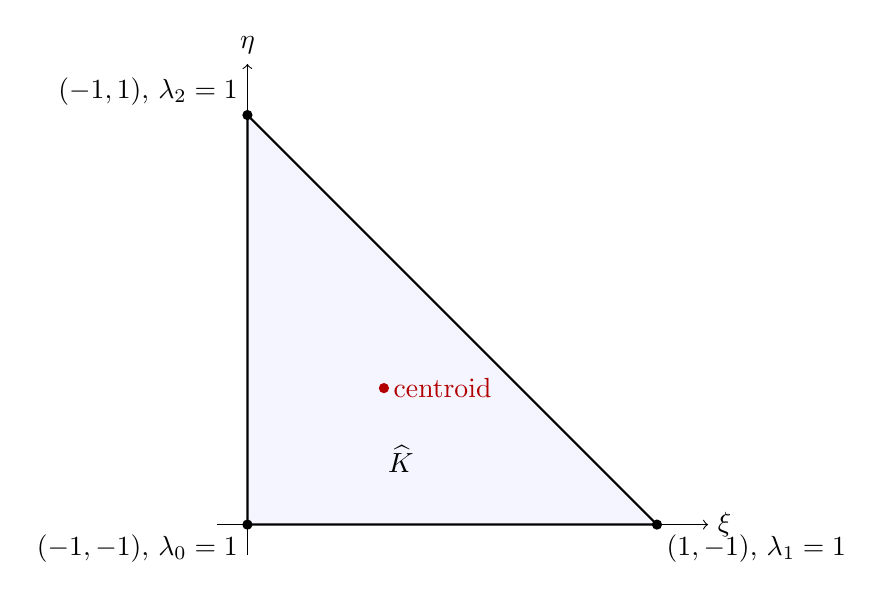
\begin{tikzpicture}[scale=2.6]
  \coordinate (A) at (0,0);
  \coordinate (B) at (2,0);
  \coordinate (C) at (0,2);
  \fill[blue!4] (A) -- (B) -- (C) -- cycle;
  \draw[thick] (A) -- (B) -- (C) -- cycle;
  \fill (A) circle (0.025) node[below left] {\((-1,-1)\), \(\lam_0=1\)};
  \fill (B) circle (0.025) node[below right] {\((1,-1)\), \(\lam_1=1\)};
  \fill (C) circle (0.025) node[above left] {\((-1,1)\), \(\lam_2=1\)};
  \draw[->] (-0.15,0) -- (2.25,0) node[right] {\(\xi\)};
  \draw[->] (0,-0.15) -- (0,2.25) node[above] {\(\eta\)};
  \fill[red!70!black] (0.6667,0.6667) circle (0.025) node[right] {centroid};
  \node at (0.75,0.32) {\(\Khat\)};
\end{tikzpicture}
\caption{The reference triangle used by \code{hybridge/core/quadrature.py}.}
\label{fig:reference-triangle}
\end{figure}

\section{\texorpdfstring{Why degree \(2p\) is the target}{Why degree 2p is the target}}

For diffusion and reaction with constant coefficients, the local reference
volume tensors contain integrals of the form
\[
  M_{ij} = \int_{\Khat} \phi_i\phi_j\,\dd x,
  \qquad
  S_{ij} = \int_{\Khat} \grad\phi_i\cdot\grad\phi_j\,\dd x.
\]
If \(\phi_i,\phi_j\in\Phat_p(\Khat)\), then
\[
  \phi_i\phi_j\in\Phat_{2p}(\Khat),
  \qquad
  \grad\phi_i\cdot\grad\phi_j\in\Phat_{2p-2}(\Khat).
\]
Thus a triangle quadrature rule exact for every polynomial in
\(\Phat_{2p}\) is enough for exact mass and stiffness matrices in exact
arithmetic.  It is also enough to integrate every single basis function in
\(\Phat_{2p}\).

This statement is about polynomial degree.  It does not cover all possible HDG
terms.  If a coefficient is itself represented by a degree-\(p\) field, then
\[
  c_h\,\phi_i\phi_j \in \Phat_{3p}(\Khat),
\]
so a degree-\(2p\) rule is no longer guaranteed to be exact for that weighted
mass term.

\section{Basis formulas}

The implementations are in \code{hybridge/core/basis.py}.  The three supported
element basis families span the same polynomial space \(\Phat_p(\Khat)\), but
they are evaluated by different formulas.

\subsection{Bernstein basis}

For nonnegative integers \(i,j,k\) with \(i+j+k=p\), the Bernstein basis is
\[
  B_{ijk}^{(p)}(\xi,\eta)
  =
  \frac{p!}{i!\,j!\,k!}
  \lam_0^i\lam_1^j\lam_2^k.
\]
The barycentric gradients are constant:
\[
  \grad\lam_0=\left(-\frac12,-\frac12\right),\qquad
  \grad\lam_1=\left(\frac12,0\right),\qquad
  \grad\lam_2=\left(0,\frac12\right).
\]
This is the simplest case: the formulas are visibly polynomials in
\((\xi,\eta)\).

\subsection{\texorpdfstring{Hierarchical \(C^0\) basis}{Hierarchical C0 basis}}

The legacy hierarchical \(C^0\) basis uses the collapsed coordinate
\[
  a = \frac{2(1+\xi)}{1-\eta}-1,
\]
and the one-dimensional linear factors
\[
  e_-=\frac{1-a}{2},\qquad e_+=\frac{1+a}{2},\qquad
  y_-=\frac{1-\eta}{2},\qquad y_+=\frac{1+\eta}{2}.
\]
Let \(P_n^{(\alpha,\beta)}\) denote a Jacobi polynomial.  For a fixed total
order \(p\), the vertex modes are
\[
  \psi_{0,0}=e_-y_-,
  \qquad
  \psi_{p,0}=e_+y_-,
  \qquad
  \psi_{0,p}=y_+.
\]
The edge modes are
\[
  \psi_{m,0}
  =
  e_-e_+\,P_{m-1}^{(1,1)}(a)\,y_-^{m+1},
  \qquad 1\le m\le p-1,
\]
\[
  \psi_{m,p-m}
  =
  e_+\,y_-y_+\,P_{p-m-1}^{(1,1)}(\eta),
  \qquad 1\le m\le p-1,
\]
\[
  \psi_{0,n}
  =
  e_-\,y_-y_+\,P_{n-1}^{(1,1)}(\eta),
  \qquad 1\le n\le p-1.
\]
For interior modes \(m\ge1\), \(n\ge1\), and \(m+n<p\),
\[
  \psi_{m,n}
  =
  e_-e_+\,P_{m-1}^{(1,1)}(a)\,
  y_-^{m+1}\,y_+\,
  P_{n-1}^{(2m-1,1)}(\eta).
\]
The formula contains \(a=(2(1+\xi))/(1-\eta)-1\), so its derivatives contain
factors like \((1-\eta)^{-1}\).  At the top vertex \((-1,1)\), these are
removable singularities in the polynomial being represented.  The code has a
special branch near that vertex.  The new tests make sure interior Dunavant
points and near-vertex probe points produce finite basis and gradient values.

\subsection{Dubiner-style basis}

The Dubiner-style basis also uses the collapsed coordinate \(a\), together
with \(\eta\).  For indices \(m,n\ge0\) with \(m+n\le p\),
\[
  D_{m,n}(\xi,\eta)
  =
  P_m^{(0,0)}(a)
  \left(\frac{1-\eta}{2}\right)^m
  P_n^{(2m+1,0)}(\eta).
\]
The factor \(((1-\eta)/2)^m\) cancels the apparent singularity introduced by
the collapsed coordinate.  At \((-1,1)\), the implementation uses the limiting
value
\[
  D_{0,n}(-1,1)=n+1,\qquad D_{m,n}(-1,1)=0\quad(m>0).
\]
Again, the mathematical functions are polynomials on \(\Khat\); the numerical
care is in evaluating them near the collapsed vertex.

\section{Symmetric triangle quadrature}

The test module uses compact Dunavant rules through exact degree \(12\).  A
symmetric rule is most easily stored in barycentric orbits:
\[
  \operatorname{orb}(a,b,b)
  =
  \{(a,b,b),(b,a,b),(b,b,a)\},
\]
and, when all entries differ,
\[
  \operatorname{orb}(a,b,c)
  =
  \{(a,b,c),(a,c,b),(b,a,c),(b,c,a),(c,a,b),(c,b,a)\}.
\]
The quadrature formula used by the test is
\[
  \int_{\Khat} f(\xi,\eta)\,\dd x
  \approx
  2\sum_q w_q^{\mathrm{unit}}\,
  f\!\left(-1+2\lam_{q,1},-1+2\lam_{q,2}\right),
\]
where \(w_q^{\mathrm{unit}}\) are weights tabulated for a unit-area triangle.

\begin{table}[htbp]
\centering
\begin{tabular}{rrrr}
\toprule
HDG order \(p\) & Required exact degree \(2p\) & Dunavant points & Duffy points with \(n=2p\) \\
\midrule
1 & 2  & 3  & 4 \\
2 & 4  & 6  & 16 \\
3 & 6  & 12 & 36 \\
4 & 8  & 16 & 64 \\
5 & 10 & 25 & 100 \\
6 & 12 & 33 & 144 \\
\bottomrule
\end{tabular}
\caption{Point counts for exact integration through degree \(2p\). The Duffy
column is the collapsed tensor-product pattern when the one-dimensional count
is set to \(2p\).}
\label{tab:point-counts}
\end{table}

\begin{figure}[htbp]
\centering
\begin{tikzpicture}[x=0.85cm,y=0.08cm]
  \draw[->] (0,0) -- (7,0) node[right] {\(p\)};
  \draw[->] (0,0) -- (0,38) node[above] {points};
  \foreach \x in {1,2,3,4,5,6} {
    \draw (\x,0) -- (\x,-1.2) node[below] {\x};
  }
  \foreach \y in {0,10,20,30} {
    \draw (0,\y) -- (-0.12,\y) node[left] {\y};
  }
  \draw[blue!65!black,thick] (1,3) -- (2,6) -- (3,12) -- (4,16) -- (5,25) -- (6,33);
  \foreach \x/\y in {1/3,2/6,3/12,4/16,5/25,6/33} {
    \fill[blue!65!black] (\x,\y) circle (0.08);
  }
  \draw[red!70!black,dashed,thick] (1,4) -- (2,16) -- (3,36) -- (4,64) -- (5,100) -- (6,144);
  \node[blue!65!black,right] at (6,33) {Dunavant};
  \node[red!70!black,right] at (2.8,32) {Duffy \(n^2\)};
\end{tikzpicture}
\caption{The symmetric rule grows much more slowly in point count than the
collapsed tensor-product Duffy rule.  The red curve is clipped by the vertical
axis range after \(p=3\); its \(p=6\) value is \(144\).}
\label{fig:point-growth}
\end{figure}

\section{Test matrix}

The host tests are deliberately independent of the GPU assembly path.  They
use NumPy and Numba only.

\subsection{Monomial exactness}

For each available Dunavant rule with declared exact degree
\[
  d\in\{2,4,6,8,10,12\},
\]
the tests integrate every monomial
\[
  \xi^r\eta^s,\qquad r+s\le d,
\]
and compare against the exact integral over \(\Khat\).  The exact integral is
computed by expanding through barycentric simplex moments:
\[
  \int_{\Khat}\xi^r\eta^s\,\dd x
  =
  4\sum_{i=0}^{r}\sum_{j=0}^{s}
    \binom{r}{i}\binom{s}{j}
    (-1)^{r-i+s-j}2^{i+j}
    \frac{i!\,j!}{(i+j+2)!}.
\]

\subsection{\texorpdfstring{Basis exactness in \(\Phat_{2p}\)}{Basis exactness in P2p}}

For each \(p=1,\ldots,6\) and each basis type
\[
  \code{bernstein},\qquad \code{hier_C0},\qquad \code{dub_orth},
\]
the tests build the full basis for \(\Phat_{2p}\), integrate every basis mode
with the degree-\(2p\) Dunavant rule, and compare the result to a high-order
Duffy reference:
\[
  \sum_q w_q^{D}\phi_i(x_q^D)
  \approx
  \sum_q w_q^{H}\phi_i(x_q^H).
\]
This is the direct check requested for exactness of all basis functions of
degree \(2p\), not only monomials.

\subsection{Mass and stiffness matrices}

For each \(p=1,\ldots,6\), the tests tabulate \(\Phat_p\) basis values and
gradients at the degree-\(2p\) Dunavant nodes.  They assemble
\[
  M_{ij}^{D} = \sum_q w_q^D\phi_i(x_q^D)\phi_j(x_q^D),
\]
and
\[
  S_{ij}^{D} =
  \sum_q w_q^D
  \grad\phi_i(x_q^D)\cdot\grad\phi_j(x_q^D).
\]
They compare these matrices with high-order Duffy matrices built through the
same reference-data constructor used by the solver.  They also compare a
direct NumPy assembly with a simple host Numba loop so that future raw-kernel
experiments have a clear scalar reference.

\subsection{ReferenceElementData consistency}

The tests also check that \code{hybridge/core/quadrature.py} computes its cached
reference tensors consistently.  For each \(p=0,\ldots,6\) and each basis, the
test rebuilds and compares:
\begin{itemize}[nosep]
  \item the volume mass matrix \code{MKrf};
  \item \code{MKrf_inv};
  \item \code{weighted_phi}, \code{weighted_phi_phi_flat}, and
        \code{weighted_triple_phi_flat};
  \item the edge mass \code{M_rf_fc};
  \item face coupling tables and their legacy aliases.
\end{itemize}
This confirms internal tensor consistency for the selected
\code{ReferenceElementData} rule, but it does not replace independent
monomial and basis exactness tests.

\section{Validation execution}

Automated checks live in
\code{tests/test_symmetric_triangle_quadrature_host.py}. They cover monomial
exactness, basis integration, mass and stiffness matrices, and cached reference
tensors. Pass counts and wall times belong to release evidence rather than this
derivation.

\section{Implementation policy}

For orders \(p\leq 6\), a positive interior Dunavant rule exact through degree
\(2p\) needs at most \(33\) volume points, compared with \(144\) points for a
collapsed Duffy rule with \code{volume_quad_1d=12}. The automatic policy uses
compact tabulated Dunavant rules through polynomial order 7 and then selects
the lower-point admissible fallback. The generated positive-weight symmetric
rule remains explicit, while the collapsed Duffy rule remains available for
compatibility and higher-order fallback.

\section{References}

\begin{enumerate}[label={[\arabic*]},leftmargin=*]
  \item D. A. Dunavant, ``High Degree Efficient Symmetrical Gaussian
        Quadrature Rules for the Triangle,'' \emph{International Journal for
        Numerical Methods in Engineering}, 21, 1129--1148, 1985.
  \item J. N. Lyness and D. Jespersen, ``Moderate Degree Symmetric Quadrature
        Rules for the Triangle,'' \emph{IMA Journal of Applied Mathematics},
        15, 19--32, 1975.
  \item John Burkardt, Dunavant triangle rule archive:
        \url{https://people.sc.fsu.edu/~jburkardt/f_src/triangle_dunavant_rule/triangle_dunavant_rule.html}.
  \item Local code references:
        \code{hybridge/core/basis.py},
        \code{hybridge/core/quadrature.py}, and
        \code{tests/test_symmetric_triangle_quadrature_host.py}.
\end{enumerate}

\end{document}
